% !TeX program = xelatex
\documentclass[9pt]{beamer}
\usepackage{xcolor}
\definecolor{orange}{HTML}{71697A}
\definecolor{lightgray}{HTML}{CCCCCC}
\definecolor{red}{HTML}{AC454A}
\definecolor{brown}{HTML}{EAD296}
\definecolor{darkgrey}{HTML}{313630}
\definecolor{cornflower}{HTML}{247BA0}
\definecolor{sienna}{HTML}{6C464F}
\usefonttheme{professionalfonts} % using non standard fonts for beamer
\usefonttheme{serif} % default family is serif
\usepackage{fontspec}
\usepackage{setspace}
\usepackage{natbib}
\usepackage{animate}
\usepackage{graphicx}
%\usepackage[T1]{fontenc}

\bibliographystyle{abbrv}
%\setmainfont{Liberation Serif}
%\setmainfont{Liberation Serif}
\setmainfont{Comfortaa}
%\usepackage[T1]{fontenc}

\setbeamercolor{frametitle}{bg=orange,fg=white}
\setbeamercolor{author in head/foot}{bg=orange,fg=white}

%\setbeamerfont{page number}{size=\Huge}

%\setbeamertemplate{itemize itemjpegs}[circle]
\useinnertheme{circles}
\setbeamercolor{palette primary}{bg=orange,fg=white}
%\setbeamercolor{palette secondary}{bg=red,fg=white}
\setbeamertemplate{itemize item}{\color{darkgrey}$\circ$}
\setbeamercolor{structure}{fg=darkgrey} % itemize, enumerate, etc

%\setbeamercolor{section in head/foot}{bg=red}
\setbeamercolor{title}{fg=orange} %, bg=brown
\setbeamercolor{author}{fg=darkgrey}
\setbeamercolor{institute}{fg=darkgrey}
\setbeamercolor{date}{fg=darkgrey}
%\setbeamercolor{normal text}{fg=darkgrey}
\makeatletter
\setbeamertemplate{headline}{%
	\usebeamercolor[bg]{frametitle}\rule{\textwidth}{1cm}
}
\setbeamerfont{title}{size=\LARGE}
\setbeamerfont{institute}{size=\normalsize}
\renewcommand*{\bibfont}{\scriptsize}


\setbeamertemplate{frametitle}{%
	\vskip-1cm%
	\begin{minipage}[c][\headheight][c]{\textwidth}%
		\usebeamerfont{frametitle}
		\strut\insertframetitle\par
		{%
			\ifx\insertframesubtitle\@empty%
			\else%
			{\usebeamerfont{framesubtitle}\usebeamercolor[fg]{framesubtitle}\strut\insertframesubtitle\par}%
			\fi
		}%      
		\vspace*{0.05cm}
	\end{minipage}%
	\vskip-0.1em
}
%\setbeamertemplate{footline}{%
%	\leavevmode%
%	\hbox{\begin{beamercolorbox}[wd=\paperwidth,ht=4.5ex,dp=3.125ex]{author in head/foot}%
%			\usebeamerfont{author in head/foot} bar
%	\end{beamercolorbox}}%
%	\vskip0pt%
%}
\makeatother


\title{The Interactive Isnalyser \\
	\small Automation of isnād trees drawing}
\author{Maroussia Bednarkiewicz, Álvaro Tejero-Cantero, Stefan Wezel}
\institute{mlcolab @ Tübingen University Cluster of Excellence}

\date{\today}


%\setbeamertemplate{sidebar right}{}
%\setbeamertemplate{footline}{%
%	\hfill\usebeamertemplate***{navigation symbols}
%	\hspace{1cm}\insertframenumber{}}
\setbeamerfont{page number in head/foot}{size=\small}
    \setbeamertemplate{footline}{%
	\raisebox{5pt}{\makebox[\paperwidth]{\hfill\makebox[10pt]{\scriptsize\insertframenumber}}}}
\setbeamertemplate{navigation symbols}{}
%\onehalfspacing
\setstretch{1.3}
\begin{document}
	

\setbeamercolor{background canvas}{bg=white}
\setbeamercolor{normal text}{fg=darkgrey}
\usebeamercolor[fg]{normal text}
\begin{frame}[plain]
	\titlepage
\end{frame} 



\setbeamercolor{background canvas}{bg=white}
\setbeamercolor{normal text}{fg=darkgrey}
\usebeamercolor[fg]{normal text}
\setbeamertemplate{itemize item}{\color{darkgrey}$\circ$}
\begin{frame}
\frametitle{Setting}
\framesubtitle{Transmission of Oral Tradition}
\begin{itemize}%\setlength\itemsep{1.5em}
%	\item Tour through this project
%	\item But before
%	\item Ḥadīth
	\item Scholars model Ḥadīth transmissions with isnād trees
	\item Drawing by hand can be tedious
	\item Automatization approaches
	\begin{itemize}
		\item Automation of data processing
		\item Automation of visualization (ours)
	\end{itemize}
	\item Our focus:
	\begin{itemize}
		\item Reproducability
		\item Open source spirit -> improvability
		\item Colaborative platform
	\end{itemize}
	\item Two steps
	\begin{itemize}
		\item Software library (Python)
		\item Web application (Javascript)
	\end{itemize}
%	\item Visualization helps
\end{itemize}
%image here
\end{frame} 





\begin{frame}
\frametitle{Isnalyser}
\framesubtitle{The beginnings}
\begin{figure}
	%	\flushright
	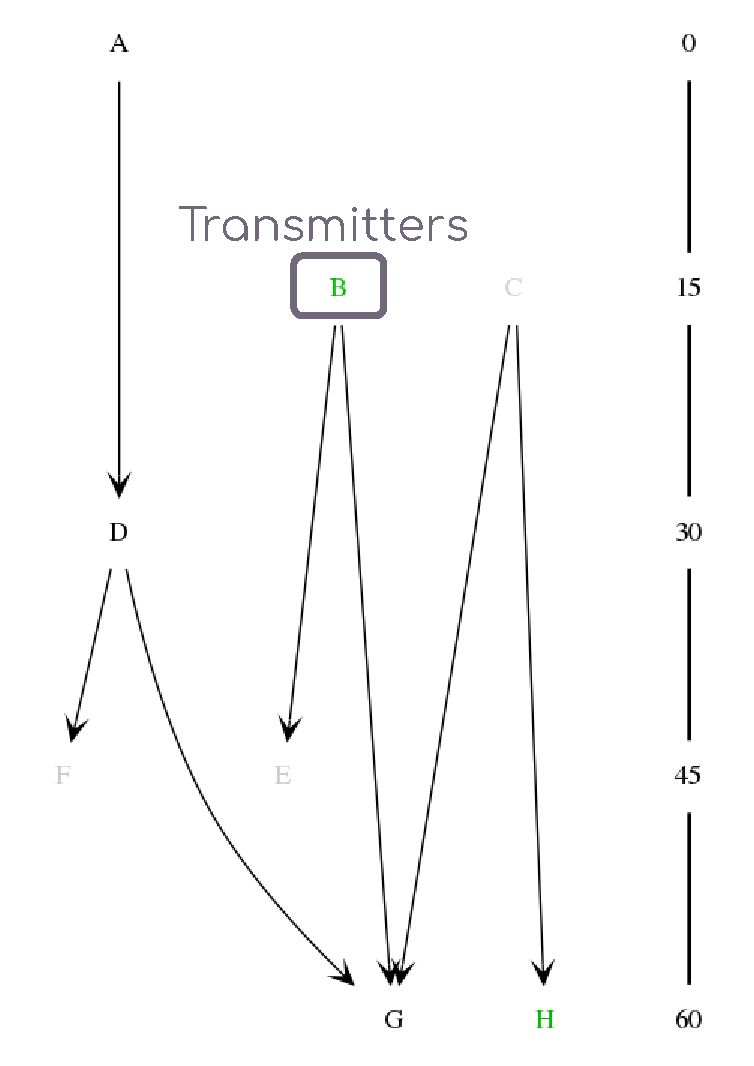
\includegraphics[width=.5\linewidth]{figures/isnalyser_parts_1.pdf}
\end{figure}
\end{frame} 
\begin{frame}
\frametitle{Isnalyser}
\framesubtitle{The beginnings}
\begin{figure}
	%	\flushright
	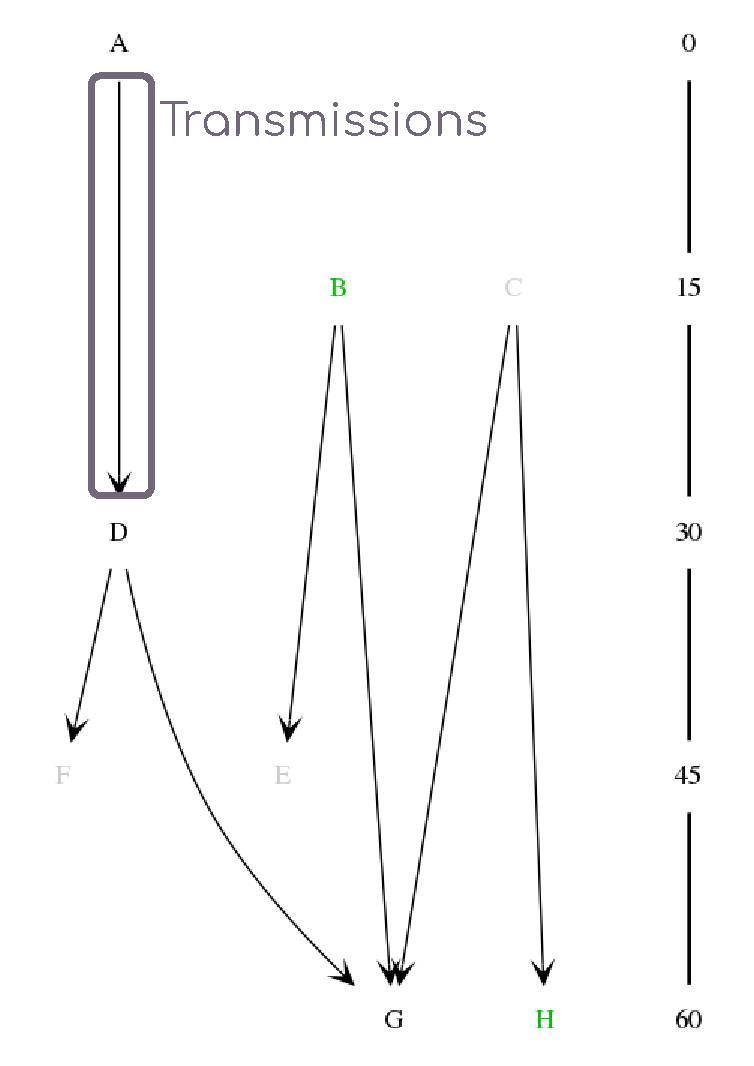
\includegraphics[width=.5\linewidth]{figures/isnalyser_parts_2.pdf}
\end{figure}
\end{frame} 
\begin{frame}
\frametitle{Isnalyser}
\framesubtitle{The beginnings}
\begin{figure}
	%	\flushright
	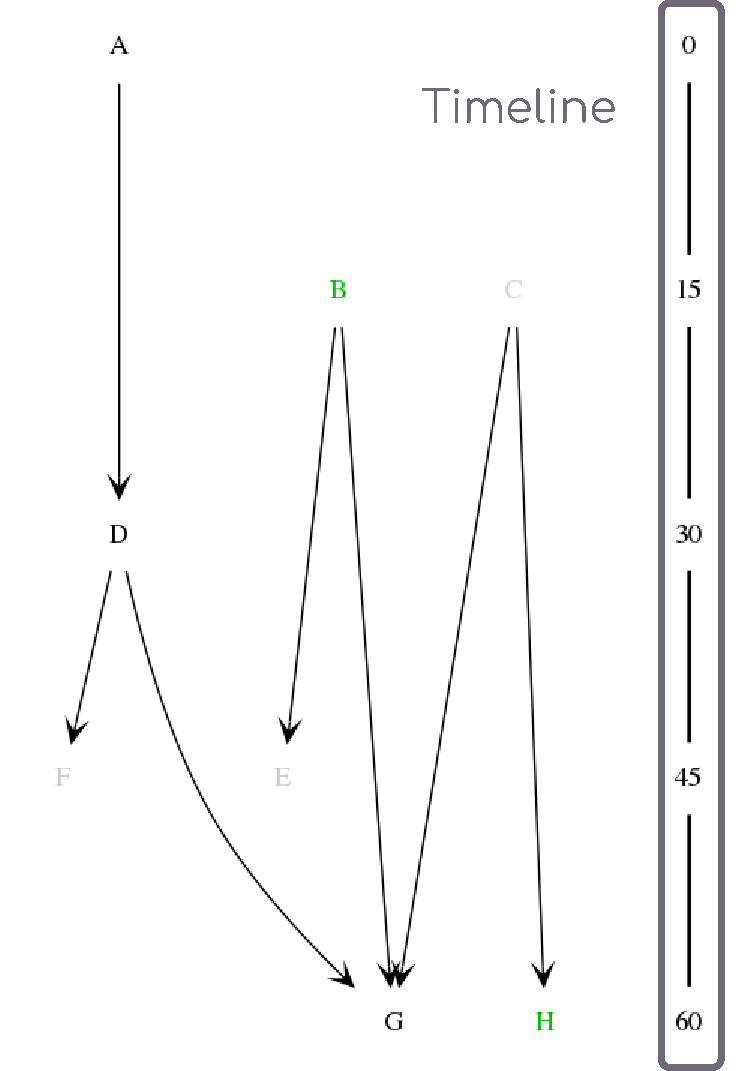
\includegraphics[width=.5\linewidth]{figures/isnalyser_parts_3.pdf}
\end{figure}
\end{frame} 
\begin{frame}
\frametitle{Isnalyser}
\framesubtitle{The beginnings}
\begin{itemize}%\setlength\itemsep{1.5em}
	\item Exploring different tools/languages
	\item Python as language of choice
	\begin{itemize}
		\item Powerful and flexible
		\item Great community and ecosystem
		\item Graphviz as library for drawing graphs
	\end{itemize}
	\item Graphviz
	\begin{itemize}
		\item Open source tool
		\item Draws graphs specified in DOT language
		\item Available as Python library
	\end{itemize}
	%	\item Basic constraints
\end{itemize}
%	\begin{figure}
%%	\flushright
%	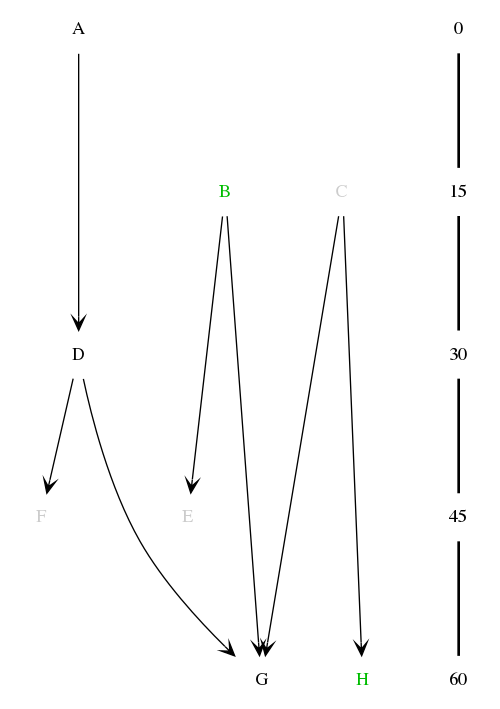
\includegraphics[width=.28\linewidth]{figures/graphviz.png}
%\end{figure}
\end{frame} 








\begin{frame}
\frametitle{Isnalyser}
\framesubtitle{Creating the library}
\begin{itemize}%\setlength\itemsep{1.5em}
		\item Next step: create Open source Python library from code 
		\begin{itemize}
			
	\item Move everything to Github%(first step towards open source project)
	\item PyPI as platform for Python libraries
	\item Adjust folder/file structure according to PyPI standards
	\item Register on Test PyPI and PyPI
	\begin{figure}
		\flushleft
		
\includegraphics[width=.6\linewidth]{figures/test_pypi.png}
	\end{figure}
	\item Upload on Test PyPI
	\begin{itemize}
		\item See if it works
		\item See that is does not work
		\item Repeat 3-4 times until it works
	\end{itemize}
	\item Upload to real PyPI and feel good!
\end{itemize}
		\end{itemize}
\end{frame} 


\begin{frame}
\frametitle{Isnalyser}
\framesubtitle{Publishing the library}
	\begin{figure}
	\flushleft
	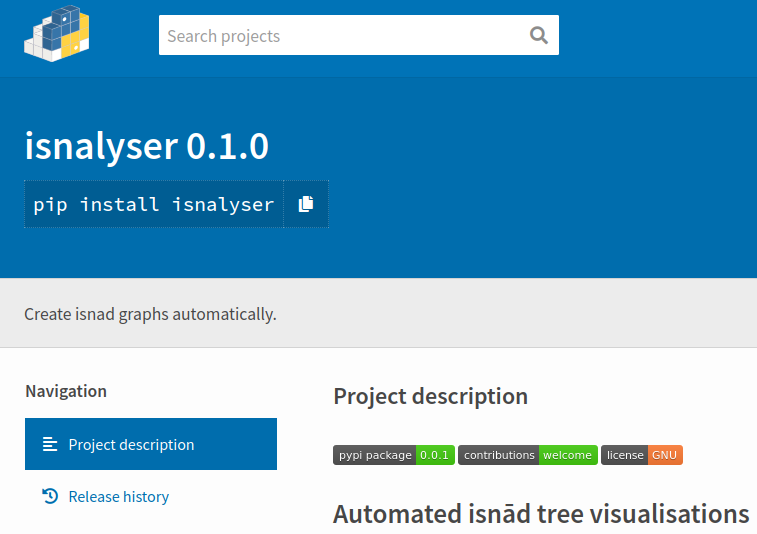
\includegraphics[width=.6\linewidth]{figures/pypi.png}
\end{figure}
\begin{itemize}%\setlength\itemsep{1.5em}
%	\item Ready for use
	\item If you are interested: Just \texttt{pip install isnalyser}
	\item Documentation on Github
\end{itemize}
\end{frame} 



\begin{frame}
\frametitle{Isnalyserjs}
\framesubtitle{Making the isnalyser more accessible}
\begin{itemize}%\setlength\itemsep{1.5em}
	\item Python is great but requires coding knowledge
	\item Limited audience/reproducability?
	\item Idea: create a web application
	\item Users can upload table and explore their data
	\item Natural choice: Javascript
\end{itemize}
	\begin{figure}
%	\flushleft
	
\includegraphics[width=.6\linewidth]{figures/python2js.pdf}
\end{figure}
\end{frame} 



\begin{frame}
\frametitle{Isnalyserjs}
\framesubtitle{Choosing the tools}
\begin{itemize}%\setlength\itemsep{1.5em}
	\item But which extensions?
	\item Long phase of exploration
	\begin{itemize}
		\item D3, Dagre, Cytoscape, ...
	\end{itemize}
	\begin{figure}
	\flushleft
	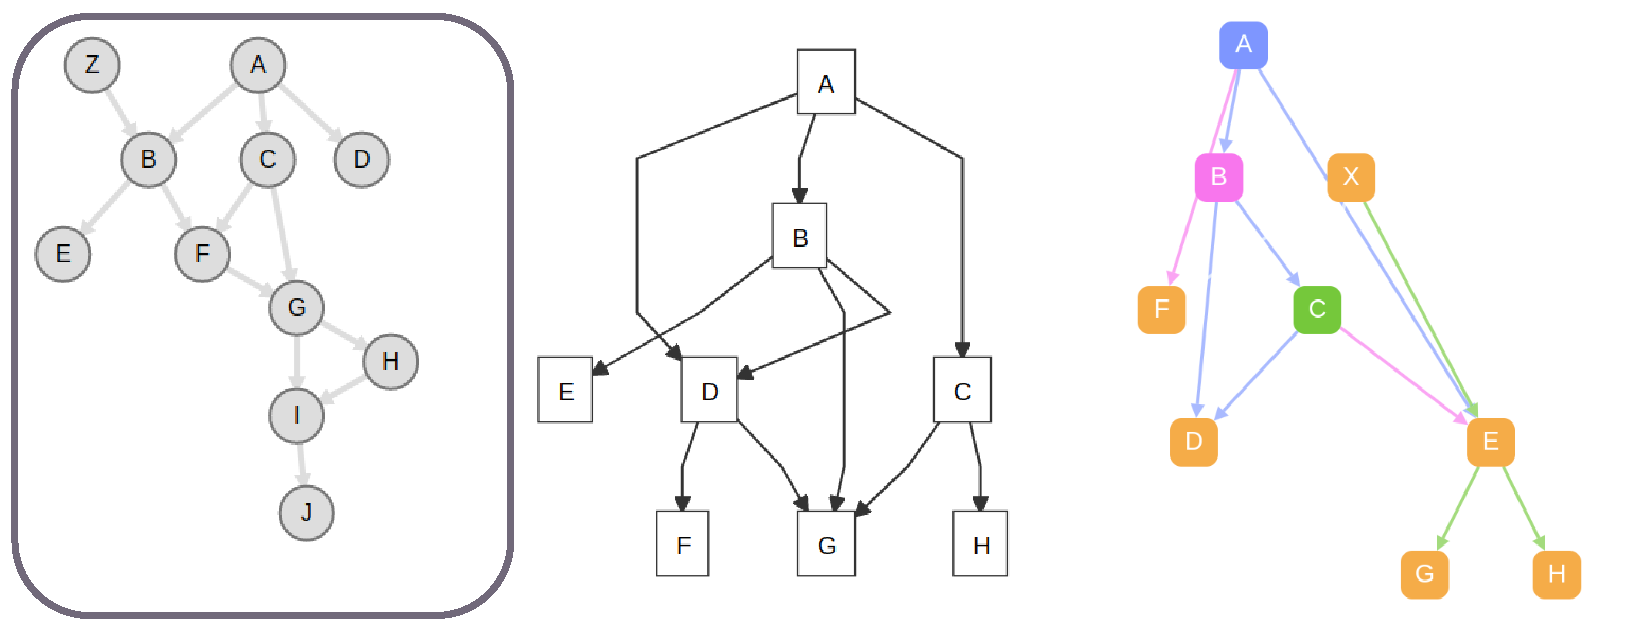
\includegraphics[width=1\linewidth]{figures/js_libs_1.pdf}
\end{figure}
\end{itemize}
\end{frame} 
\begin{frame}
\frametitle{Isnalyserjs}
\framesubtitle{Choosing the tools}
\begin{itemize}%\setlength\itemsep{1.5em}
	\item But which extensions? Not just the same
	\item Long phase of exploration
	\begin{itemize}
		\item D3, Dagre, Cytoscape, ...
	\end{itemize}
	\begin{figure}
		\flushleft
		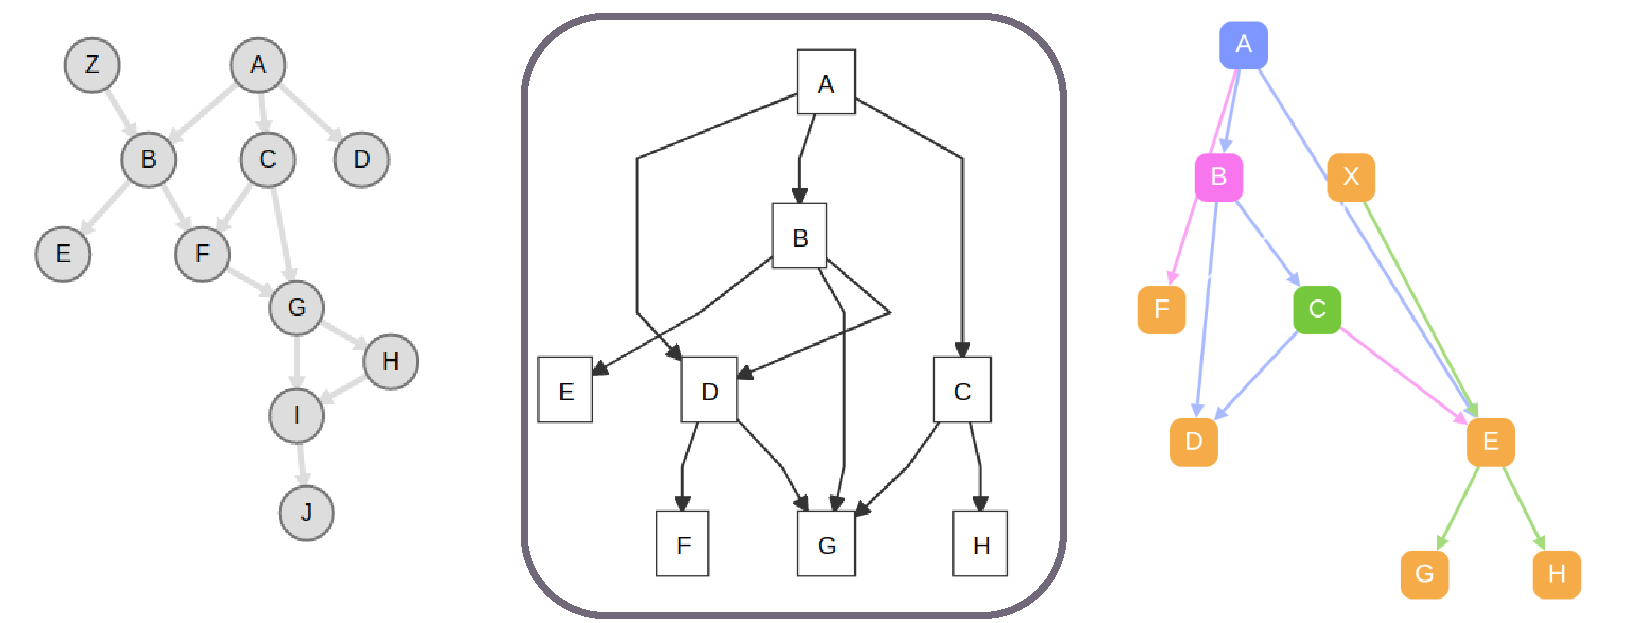
\includegraphics[width=1\linewidth]{figures/js_libs_2.pdf}
	\end{figure}
\end{itemize}
\end{frame} 
\begin{frame}
\frametitle{Isnalyserjs}
\framesubtitle{Choosing the tools}
\begin{itemize}%\setlength\itemsep{1.5em}
	\item But which extensions?
	\item Long phase of exploration
	\begin{itemize}
		\item D3, Dagre, Cytoscape, ...
	\end{itemize}
	\begin{figure}
		\flushleft
		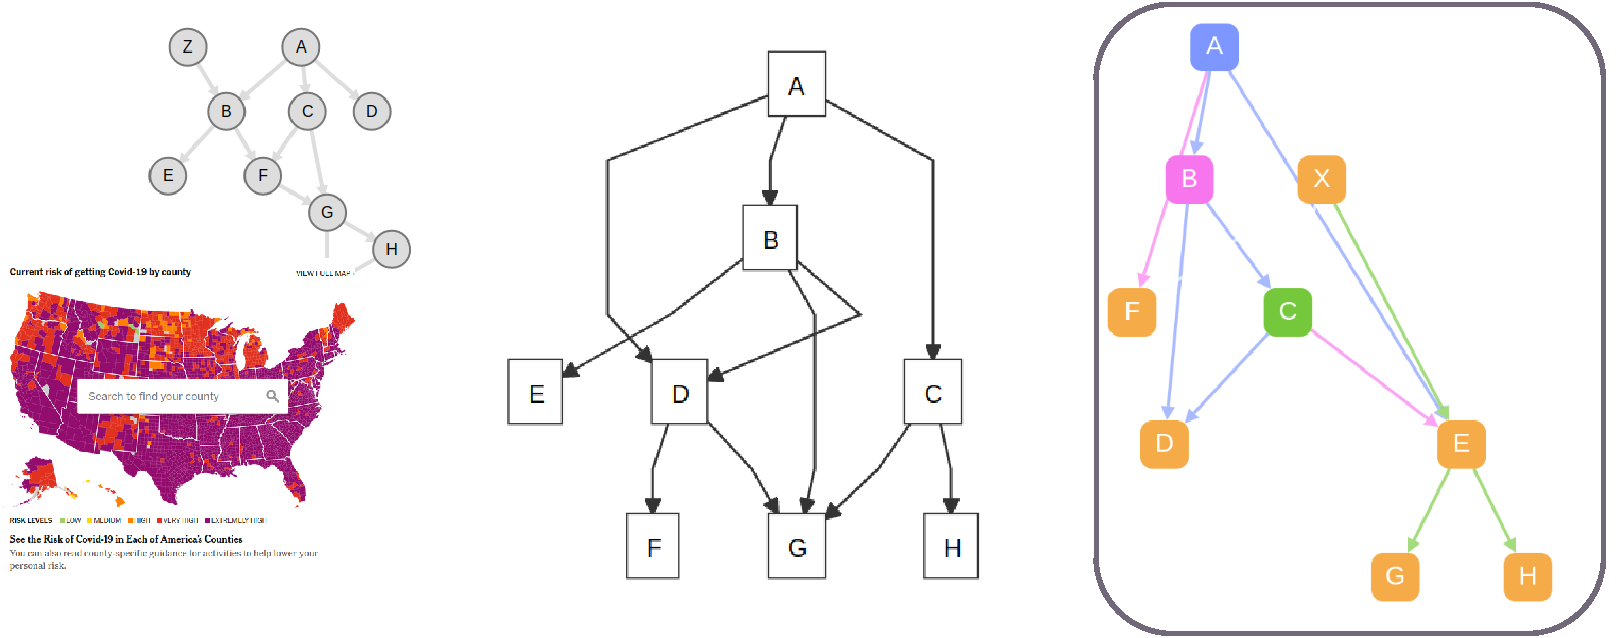
\includegraphics[width=1\linewidth]{figures/js_libs_3.pdf}
	\end{figure}
\end{itemize}
\end{frame} 


\begin{frame}
\frametitle{Isnalyserjs}
\framesubtitle{Choosing the tools}
\begin{itemize}%\setlength\itemsep{1.5em}
%	\item Each has strengths and weaknesses
	\item Graphviz has good layout and constraint capabilities
	\item Solution: d3-graphviz
	\begin{itemize}
		\item Direct translations of Graphviz to Javascript with d3-capabilities
		\item Combine graphviz layout and d3 visualization/interaction 
		\item Interactive graph with nice layout
	\end{itemize}
\end{itemize}
	\begin{figure}
	\flushright
	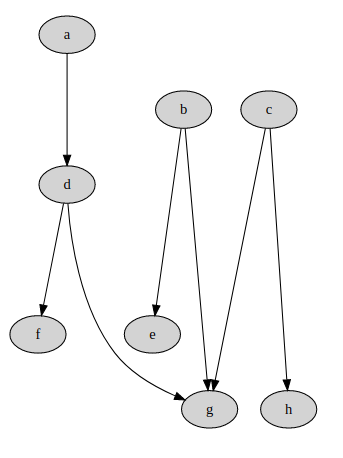
\includegraphics[width=.42\linewidth]{figures/d3_graphviz.png}
\end{figure}
\end{frame} 


\begin{frame}
\frametitle{Isnalyserjs}
\framesubtitle{Getting to work}
\begin{itemize}%\setlength\itemsep{1.5em}
	\item Implement the functionalities from Python to Javascript
	\item Use gitflow for feature development
	\begin{itemize}
		\item Main branch
		\item Each new feature as new branch
		\item If feature is finished, merge into main branch 
	\end{itemize}
	\begin{figure}
	\flushleft
	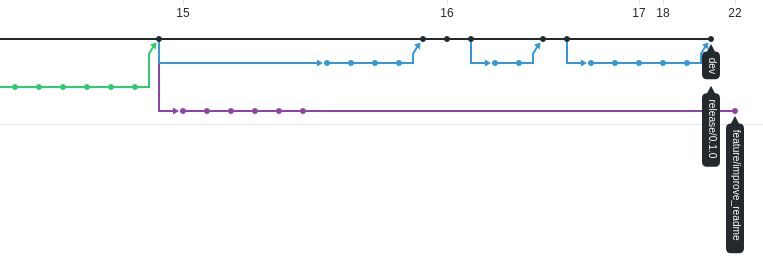
\includegraphics[width=.7\linewidth]{figures/git.png}
\end{figure}
	\item Transparent development history
	\item Always one working version
	\item Now at version 0.1.0 - ready for first release
	
%	\item Now ready for its first release
\end{itemize}
\end{frame}



\begin{frame}
\frametitle{Isnalyserjs}
\framesubtitle{}
	\begin{figure}
	\flushleft
	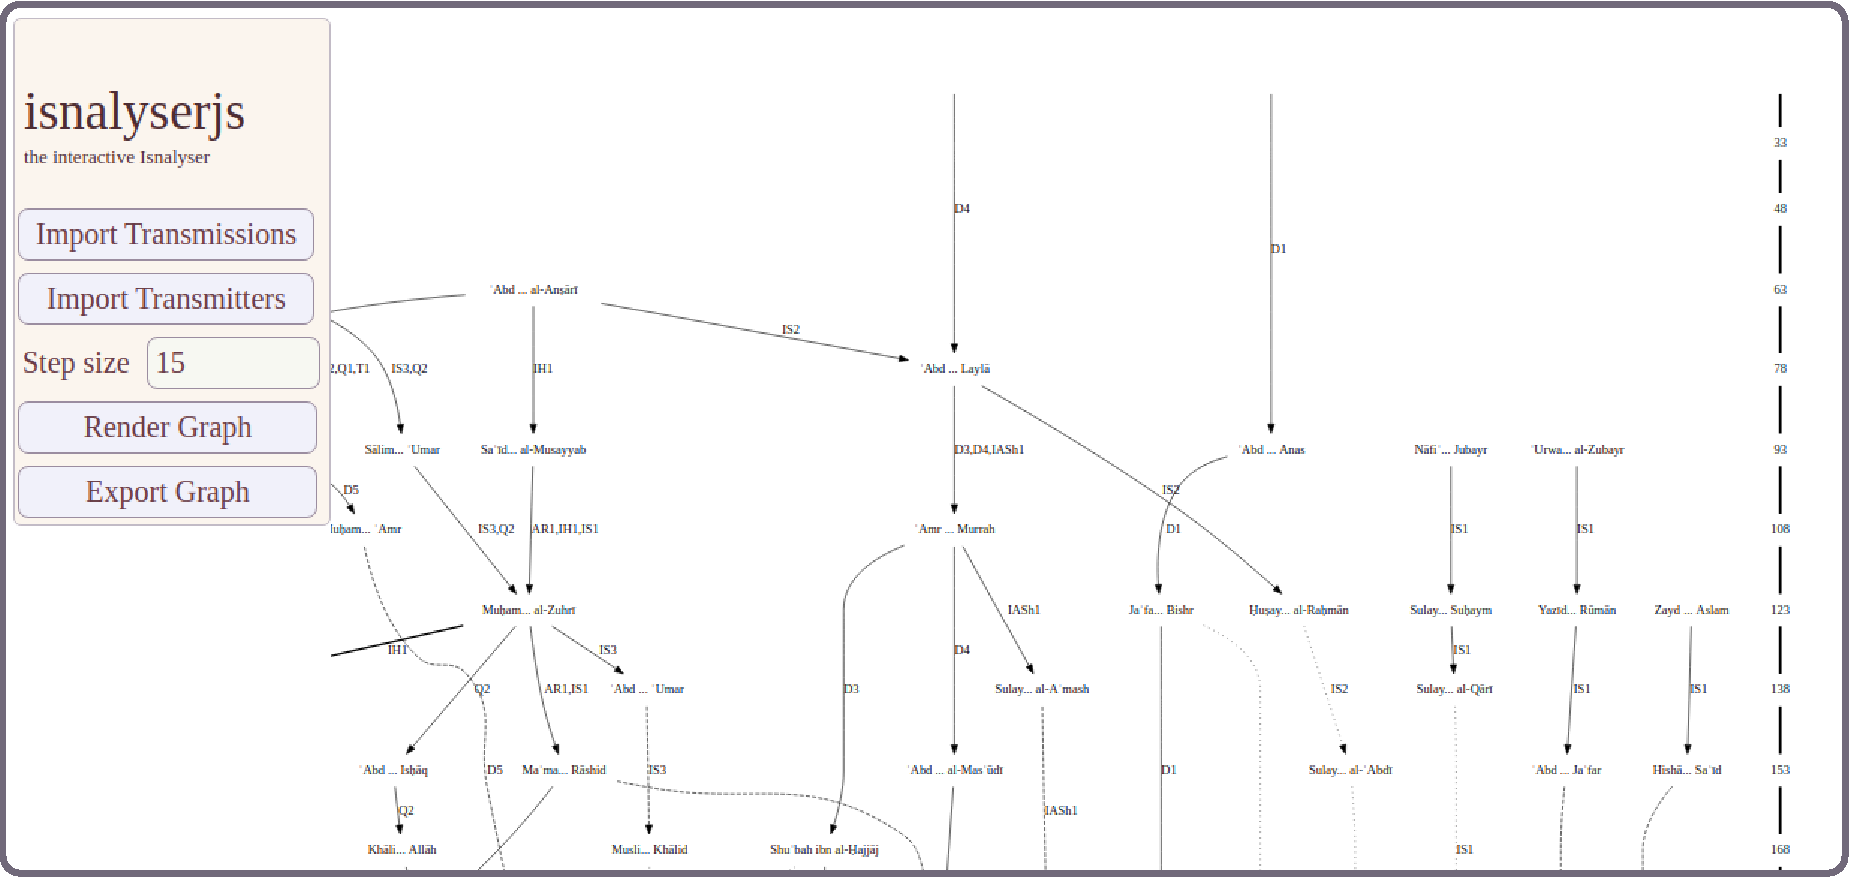
\includegraphics[width=1.1\linewidth]{figures/isnalyser_screenshot.pdf}
\end{figure}
\end{frame}



\begin{frame}
\frametitle{Future of the Isnalyser}
\framesubtitle{}
\begin{itemize}
	\item Paper in the works for Journal of Open Source Software
	\item Eventually develop into a colaborative platform
	\begin{itemize}
		\item Users can upload and share graphs
		\item Edit, annotate other's
	\end{itemize}
	\item Beyond isnād trees
	\begin{itemize}
		\item I.e. citation graphs
	\end{itemize}
\end{itemize}
\end{frame}






\setbeamercolor{background canvas}{bg=orange}
\setbeamercolor{normal text}{fg=white}
\usebeamercolor[fg]{normal text}
\setbeamertemplate{itemize item}{\color{white}$\circ$}
\setbeamercolor{structure}{fg=white} % itemize, enumerate, etc
\begin{frame}
\frametitle{Takeaways}
\framesubtitle{What did we learn from this project?}
\begin{itemize}%\setlength\itemsep{1.5em}
	\item Creating a PyPI package is not that hard
	\item Git flow helps keeping track and maintaining transparency
%	\item Know your Audience
%	\item Seemingly easy problems can turn out quite hard
%	\item Listen to different opinions %Alvaro v Maroussia v Stefan
	\item Most important part of the project are users
	\item Interaction happens on many levels
	\item If you interested in the isnalysers
	\begin{itemize}
		\item Try them out
		\item File github issues
		\item Send us mails
		\item Extent the code
	\end{itemize}
	\item Live demo
\end{itemize}
\end{frame} 








\end{document}


